% (c) 2014 Daniele Masini - d.masini.it@gmail.com
\chapter{Elementi di logica}

In questo capitolo introdurremo i concetti di base della logica e alcuni elementi che saranno utili per la lettura delle parti successive di questo testo.
La logica è ciò governa il modo di procedere nella deduzione della teoria di una qualunque disciplina scientifica e si basa su concetti elementari e intuitivi di evidente chiarezza. Quindi, partendo dalle definizioni di base se ne deducono implicazioni che portano ad accrescere la complessità della materia ma che forniscono allo studente strumenti sempre più ``potenti'' per trattare e risolvere le situazioni che gli si presenteranno nel suo corso di studi.

\section{Le proposizioni o enunciati}

Nel linguaggio comune è facile rendersi conto che alcune frasi hanno di per sé un significato che chiunque può ritenere vero o falso. Ad esempio, la frase ``il cielo è blu'' esprime un fatto che tutti ritengono vero, quindi possiamo dire che è universalmente vero. Mentre la frase ``il Sole è nero'' è considerata universalmente falsa. Esistono anche frasi che sono ritenute vere da alcuni e false da altri, come ad esempio ``Firenze è una bella città''. Ad altre frasi ancora non possiamo attribuire alcun valore di verità o falsità, come ad esempio ``Non parlare al guidatore'' o ``Fai i tuoi compiti'' o ancora ``La prossima settimana farà brutto tempo''.

\begin{definizione}
Si definisce \emph{proposizione} o \emph{enunciato} una qualunque affermazione che può essere vera o falsa.
\end{definizione}

La logica che andiamo a considerare si baserà dunque su due soli valori possibili, cioè ``vero'' e ``falso''.

\section{Cenni all'algebra degli enunciati}

Le proposizioni possono essere collegate tra loro per mezzo di opportuni operatori, in maniera del tutto analoga a quanto avviene nel linguaggio naturale per mezzo delle parole ``e'' e ``o''. Ad esempio, ``mangio una mela e cammino per strada'' e ``mangio una mela o cammino per strada''. Possiamo anche costruire una frase che ha il significato opposto a quello della frase originale utilizzando la parola ``non'', ad esempio ``non mangio una mela''.

La valutazione della verità o falsità della frase composta dipende dalla verità di ogni singola proposizione e da come esse sono collegate tra loro. Ad esempio, se sto effettivamente mangiando una mela e camminando per strada la frase ``mangio una mela e cammino per strada'' risulterà vera, ma se non sto facendo almeno una delle due cose la frase nel suo complesso risulterà falsa, poiché le singole frasi che la compongono sono collegate dalla parola ``e'' che implica che entrambe le frasi siano vere affinché la frase complessiva lo sia. La frase ``mangio una mela o cammino per strada'', invece, per la presenza della parola ``o'' risulterà vera se è effettivamente verificata almeno una delle singole frasi di cui si compone.

Per uniformare il linguaggio logico con dei simboli che abbiano un senso univoco, si utilizzeranno le seguenti convenzioni: le proposizioni saranno indicate con delle lettere come $p$ e $q$, il simbolo $\wedge$ sarà utilizzato come operatore di \emph{congiunzione logica}, che opera in maniera analoga alla parola ``e'' del linguaggio naturale, il simbolo $\vee$ sarà utilizzato come operatore di \emph{disgiunzione logica}, che funziona in maniera analoga alla parola ``o'' del linguaggio naturale, il simbolo $\neg$ sarà utilizzato come operatore di \emph{negazione logica}, con l'effetto del tutto analogo a quello della parola ``non''.
Utilizzeremo inoltre il simbolo $\Rightarrow$ per indicare l'\emph{implicazione logica} ed il simbolo $\Leftrightarrow$ per la \emph{doppia implicazione}.

Per definire il funzionamento di un operatore logico è necessario fornire la sua relativa \emph{tabella di verità} ovvero il valore (vero o falso) risultante per ogni valore vero (V) o falso (F) delle proposizioni alle quali l'operatore è applicato. Di seguito riportiamo le tabelle di verità relative agli operatori precedentemente menzionati.

\begin{center}
 % (c) 2014 Daniele Masini - d.masini.it@gmail.com
\usetikzlibrary{matrix}

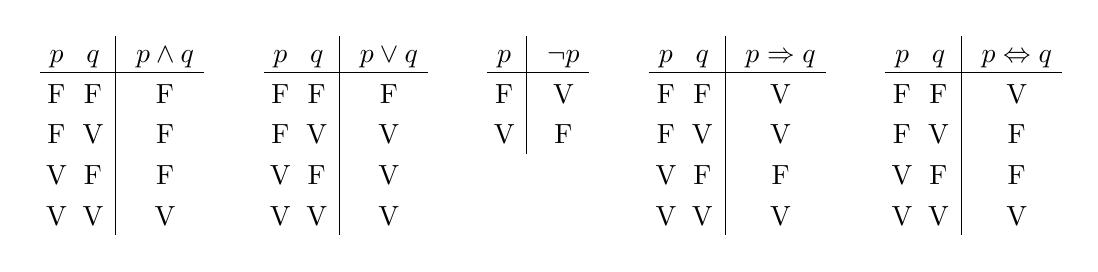
\begin{tikzpicture}
	\begin{scope}[every node/.style={anchor=base,row sep=2pt, column sep =-1pt, text depth=0pt, text height=6pt}]% ,text width=3pt
 	\matrix (tabver) [matrix of nodes]
 	{%
 		$p$ & $q$ &[-.1cm] \phantom{-} &$p \wedge q$ & [.8cm] & $p$ & $q$ &[-.1cm] \phantom{-} & $p \vee q$ &[.8cm] & $p$ &[-.1cm] \phantom{-} & $\neg p$ &[.8cm]& $p$ & $q$ &[-.1cm] \phantom{-} & $p \Rightarrow q$ &[.8cm]& $p$ & $q$ &[-.1cm] \phantom{-} & $p \Leftrightarrow q$ \\
 	 	  F   &   F    &                                 &         F           &              &  F    &  F     &                                  &         F        &           &   F    &                                 &      V&                                  &  F  &   F  &  &      V&     &  F  &   F  &  &      V\\
 	      F   &   V	  &                                 &         F           &              &   F   &  V     &                                  &         V        &           &   V   & \phantom{-}             &      F&                                  &  F  &   V  &  &      V&     &  F  &   V  &  &      F\\
 	      V   &   F	  &                                 &         F           &              &   V   &  F     &                                  &         V        &           &        &                                  &        &                                  &  V  &   F  &  &      F&     &  V  &   F  &  &      F\\
 	      V   &   V	  &\phantom{-}             &         V           &              &   V   &  V     &\phantom{-}              &         V        &           &        &                                  &        &                                  &  V  &   V  &\phantom{-}&      V&     &  V  &   V  &\phantom{-}&      V\\
 	};
	\end{scope}
	\draw (tabver-1-1.south west)--(tabver-1-4.south east);
	\draw (tabver-1-3.north)--(tabver-5-3.south);
	\draw (tabver-1-6.south west) -- (tabver-1-9.south east);
	\draw (tabver-1-8.north)--(tabver-5-8.south);
	\draw (tabver-1-11.south west) -- (tabver-1-13.south east);
	\draw (tabver-1-12.north)--(tabver-3-12.south);
	\draw (tabver-1-15.south west) -- (tabver-1-18.south east);
	\draw (tabver-1-17.north)--(tabver-5-17.south);
	\draw (tabver-1-20.south west) -- (tabver-1-23.south east);
	\draw (tabver-1-22.north)--(tabver-5-22.south);
\end{tikzpicture}

\end{center}

Le proposizioni possono anche essere tra loro in maniera più articolata, utilizzando gli operatori appena descritti ed eventualmente le parentesi per indicare quale degli operatori deve avere la precedenza di applicazione rispetto agli altri (in linea di principio l'operatore $\neg$ ha la precedenza rispetto agli altri e tutti gli altri vengono semplicemente considerati nell'ordine in cui compaiono nell'espressione, da sinistra verso destra). Da ciò ne deriva un sistema di calcolo simbolico noto anche come algebra di Boole\footnote{matematico e logico britannico (1815 - 1864).}.

\section{Dalle definizioni ai teoremi}

La teoria delle discipline scientifiche si basa su un percorso logico che, partendo dalle definizioni e dai risultati precedenti, ne individua le implicazioni e ne deduce le conseguenze. Nel corso di matematica lo studente avrà a che fare con varie tipologie di proposizioni:

\paragraph{Assiomi}
Un \emph{assioma} è una proposizione che si assume vera, senza alcuna dimostrazione. In genere sono in numero esiguo e stanno alla base della disciplina considerata.

\paragraph{Teoremi}
Un \emph{teorema} è una proposizione che riporta le conclusioni alle quali si può arrivare partendo da condizioni iniziali stabilite, per mezzo di passaggi logici successivi. \`E una proposizione del tipo\ \  $p\Rightarrow q$\ \ o\ \ $p \Leftrightarrow q$, dove la proposizione $p$ è detta \emph{ipotesi} e $q$ viene chiamata \emph{tesi}.

La \emph{dimostrazione} è il procedimento logico rigoroso che dalle condizioni iniziali indicate dal teorema (ipotesi) ne deduce le conclusioni (tesi), che quindi risultano essere la conseguenza logica delle ipotesi.
Ogni dimostrazione può essere realizzata per mezzo di vari schemi logici che possono essere di tre tipi:

\begin{itemize*}
\item \emph{dimostrazione per assurdo}: viene effettuata ritenendo vere le ipotesi e negando la tesi, verificando poi con passaggi logici che ciò porta ad un assurdo, cioè alla contraddizione delle ipotesi;
\item \emph{dimostrazione per induzione}: viene utilizzata per i teoremi relativi alle caratteristiche di elementi di insiemi numerabili. Si dimostra che il teorema vale per un determinato elemento dell'insieme (\emph{base dell'induzione}) e, ipotizzando che la tesi valga per un elemento generico (\emph{ipotesi induttiva}) si può logicamente dedurre che essa vale anche per l'elemento successivo (\emph{passo dell'induzione}). La tesi risulta così dimostrata per qualunque elemento dell'insieme;
\item \emph{dimostrazione costruttiva}: è la dimostrazione per antonomasia, ovvero quella che partendo dalle ipotesi, tramite una serie di implicazioni logiche, porta alla tesi (la maggior parte delle dimostrazioni appartengono a questa tipologia).
\end{itemize*}

Si osservi inoltre che non sempre il verificarsi della tesi di un teorema implica il verificarsi delle relative ipotesi. In generale il verificarsi delle ipotesi implica la tesi ma non viceversa. In tal caso si dice che le ipotesi sono una \emph{condizione sufficiente} per il verificarsi della tesi (implicazione logica semplice $p \Rightarrow q$). Se il verificarsi della tesi implica il verificarsi delle ipotesi si dice che le ipotesi sono una \emph{condizione necessaria} per il verificarsi della tesi (implicazione logica semplice inversa $p \Leftarrow q$, ovvero $q \Rightarrow p$). Se valgono entrambe le implicazioni cioè le ipotesi e la tesi si implicano a vicenda si dice che il verificarsi delle ipotesi è una \emph{condizione necessaria e sufficiente} al verificarsi della tesi e viceversa (doppia implicazione $p \Leftrightarrow q$).

Si consideri, ad esempio, la proposizione ``essere fiorentino significa essere toscano''.
In tal caso l'ipotesi è ``essere fiorentino'' e la tesi è ``essere toscano''. Il verificarsi dell'ipotesi implica il verificarsi della tesi, quindi la condizione ``essere fiorentino'' è sufficiente per ``essere toscano'', ma ``essere toscano'' non implica necessariamente ``essere fiorentino'', ovvero la condizione ``essere fiorentino'' è sufficiente per ``essere toscano'' ma non è necessaria.

Consideriamo, ad esempio, la proposizione ``per essere promossi bisogna avere un voto $\geq 6$ in ogni materia''.
In tal caso l'ipotesi è ``avere un voto $\geq 6$ in ogni materia'' e la tesi è ``essere promosso''. Il verificarsi dell'ipotesi implica il verificarsi della tesi, quindi la condizione ``avere un voto $\geq 6$ in ogni materia'' è sufficiente per ``essere promosso''. Ma ``essere promosso'' significa ``avere un voto $\geq 6$ in ogni materia'', ovvero la condizione ``avere un voto $\geq 6$ in ogni materia'' è anche necessaria per ``essere promosso''. Quindi la condizione ``avere un voto $\geq 6$ in ogni materia'' è necessaria e sufficiente per ``essere promosso''.

Si consideri, ad esempio, la proposizione ``per conoscere la matematica bisogna conoscere questo capitolo''.
In tal caso l'ipotesi è ``conoscere questo capitolo'' e la tesi è ``conoscere la matematica''. Il verificarsi dell'ipotesi non implica il verificarsi della tesi, quindi la condizione ``conoscere questo capitolo'' non è sufficiente per ``conoscere la matematica''. Ma ``conoscere la matematica'' significa ``conoscere questo capitolo'', ovvero la condizione ``conoscere questo capitolo'' è necessaria per ``conoscere la matematica'' ma non è sufficiente.

\paragraph{Lemmi}
La dimostrazione di un teorema può essere molto complessa e quindi in alcuni casi viene suddivisa in più parti, procedendo così per gradi nella dimostrazione di ognuna di esse. Ogni parte in cui il teorema è suddiviso, con le proprie ipotesi e tesi, è detto \emph{lemma}.

\paragraph{Corollari}
In certi casi da un teorema ne discendono direttamente altri di semplice dimostrazione. Ognuno di quest'ultimi è detto \emph{corollario} del teorema considerato.

\paragraph{Leggi o Regole}
Si tratta di teoremi che dimostrano delle caratteristiche operative, come formule, di facile applicazione o molto utilizzate da altri teoremi.


\section{Altri simboli utilizzati in matematica}

Nel linguaggio matematico si fa spesso uso di locuzioni del tipo ``per ogni \ldots'', ``esiste un \ldots'',  ``tale che \ldots''. Quindi anche nella scrittura, oltre ai simboli delle operazioni sia matematiche che logiche che man mano saranno illustrate, vengono utilizzati anche dei simboli che rappresentano in forma sintetica e in maniera univoca le espressioni precedentemente indicate. Riportiamo di seguito alcuni dei simboli che più spesso saranno utilizzati nel testo.

\begin{table}[!hb]
\begin{center}
\begin{tabular}{cl}
\toprule
Simbolo & Significato\\
\midrule
$\forall$ & per ogni \ldots{} (\emph{quantificatore universale}) \\
$\exists$ & esiste (almeno) un \ldots{} (\emph{quantificatore esistenziale}) \\
$\exists!$ & esiste un solo \ldots \\
$|$~~oppure~~$:$ & tale che \ldots \\
\bottomrule
\end{tabular}
\end{center}
\end{table}

Quindi, per esempio, la proposizione ``per ogni $a$ esiste un $b$ tale che \ldots{}'' si può scrivere in maniera simbolica~~$\forall a\;\exists b :\ldots{}$

\cleardoublepage
